\chapter{Approach}\label{chapter:approach}

\pgfplotstableread[col sep=comma]{data/sys_lit_rev.csv}\mytable

\def\printonlypositive#1{\ifnum#1>0
#1
\fi}

% Change this to one TikZ picture with one legend for all pie charts
\newcommand{\drawPie}[1]{%
  % Extract the conference name
  \pgfplotstablegetelem{#1}{Venue}\of\mytable
  \let\venue\pgfplotsretval

  % Extract the benchmark counts
  \pgfplotstablegetelem{#1}{YCSB}\of\mytable
  \let\valYCSB\pgfplotsretval

  \pgfplotstablegetelem{#1}{Sysbench}\of\mytable
  \let\valSysbench\pgfplotsretval

  \pgfplotstablegetelem{#1}{FIO}\of\mytable
  \let\valFIO\pgfplotsretval

  \pgfplotstablegetelem{#1}{OLTPBench}\of\mytable
  \let\valOLTP\pgfplotsretval

  \pgfplotstablegetelem{#1}{DBGen}\of\mytable
  \let\valDBGen\pgfplotsretval

  \begin{tikzpicture}[baseline=(current bounding box.north)]
    % Title for the conference above the pie
    \node[font=\bfseries] at (0,1.5) {\venue};

    \pie[
      /tikz/nodes={font=\footnotesize},
      color={blue!50!white, red!50!white, green!50!white, orange!50!white, purple!50!white},
      sum=auto,
      radius=1,
      text=legend,
      before number=\printonlypositive,
    ]{
      \valYCSB/YCSB,
      \valSysbench/Sysbench,
      \valFIO/FIO,
      \valOLTP/OLTPBench,
      \valDBGen/DBGen
    }
  \end{tikzpicture}
}


The goal of this thesis is to identify the most widely used frameworks for generating zipfian synthetic data in the systems programming and database community and 
make a comparative evaluation.
The first step required to achieve this is a systematic review of current approaches. The following sections describe
\begin{enumerate}
    \item the \textbf{research approach} used to identify the frameworks,
    \item the \textbf{common frameworks} recognized from the search along with short descriptions
    \item the \textbf{popularity and impact} of those tools
\end{enumerate}

% TODO : Think whether this belongs here or in evaluation
Afterwards, the \textbf{evaluation criteria} used to compare the frameworks are presented and clarified, along with a presentation of 
the tool used to compile those results.


\section{Research Approach}
To identify relevant frameworks used by the systems programming and database community, first the scope of 
venues and journals was defined. The list is comprised of:
\begin{center} % Centers the columns as a whole
    \begin{minipage}{0.8\linewidth} % Optional: restrict width for a nicer look
      \begin{multicols}{2} % Specify 2 columns
        \begin{itemize}
          \item \ac{PVLDB}
          \item \ac{SIGMOD}
          \item \ac{CIDR}
          \item \ac{OSDI}
          \item \ac{NSDI}
          \item \ac{FAST}
        \end{itemize}
      \end{multicols}
      \label{list:conferences}
    \end{minipage}
\end{center}

% TODO : How can I justify the selection of conferences here. This seems very arbitrary
These conferences were chosen due to their high selectivity and special relevancy for storage technology research, where there is a prevalence of 
standardized IO benchmarks. The search was conducted broadly following the steps indicated in \parencite{bramerSystematicApproachSearching2018}, as defined below: 
\begin{enumerate}
    \item Word search on keyword search matrix (see table~\ref{tab:keyword_search_matrix})
    \item Identify the frameworks used in the papers
    \item Extended keyword search, this time adding the frameworks identified in the previous step
\end{enumerate} 

The first step suggests the use of a keyword matrix. This works by choosing appropriate keywords
which refer to the topic of interest. Then for each such keyword, synonyms are used to improve the accuracy and scope of the search. It's defined below as:

\begin{table}[h!]
    \centering
    \begin{tabular}{|c|l|r|r|}
      \hline
       & \multicolumn{1}{c|}{Keyword 1} & \multicolumn{1}{c|}{Keyword 2} & \multicolumn{1}{c|}{Keyword 3} \\ \hline
       \parbox[t]{3mm}{\multirow{3}{*}{\rotatebox[origin=r]{90}{synonyms}}}
       & zipf   &   benchmark     &    synthetic      \\
       & zipfian   &   workload     &    generated      \\
       &    &   evaluation     &    sampled      \\
       &    &   empirical     &    sampler      \\
       &   &   dataset     &         \\ \hline
    \end{tabular}
    \caption{Keyword search matrix}
    \label{tab:keyword_search_matrix}
  \end{table} 

The columns are the keywords which are boolean OR'ed, whereas the rows are boolean AND'ed.
This means that at least one word of each column should appear in the search.

These queries where then run for the conferences and journals listed before on an unrestricted timescale. The databases consulted are
\begin{itemize}
    \item IEEE Xplore
    \item ACM Digital Library
    \item DBLP
    \item Google Scholar
\end{itemize}


\section{Common Frameworks}

On a first phase, the following frameworks were identified among the top 20 results of each conference
\begin{center}
    \begin{tabular}{|l|}
        \hline
        \textbf{Frameworks} \\ \hline\hline
        \ac{YCSB} \\ \hline
        \ac{FIO} \\ \hline
        Sysbench \\ \hline
        OLTP-Bench \cite{difallahOLTPBenchExtensibleTestbed2013} \\ \hline
        DBgen \\ \hline
    \end{tabular}
\end{center}

These frameworks were then searched with the same keyword matrix and their name as a last keyword. This has yielded the following results:

\begin{figure}[htb]
  \centering
  \begin{tabular}{ccc}
    \drawPie{0} & \drawPie{1} & \drawPie{2} \\
    \drawPie{3} & \drawPie{4} & \drawPie{5} \\
  \end{tabular}
  \caption{Pie charts for each conference (excluding Web Polygraph and pgBench).}
\end{figure}

The most popular framework by far is \textbf{YCSB}, then followed by \textbf{Sysbench} along with \textbf{FIO}. Other frameworks are
not as prevalent, but have appeared in the search results.

\subsection{Yahoo! Cloud Serving Benchmark}
\ac{YCSB} \cite{cooperBenchmarkingCloudServing2010} is a widely used benchmarking tool for cloud databases. 
It was developed by \textit{Yahoo! Research} and is now maintained by a community of developers. Its working principle is to generate workloads 
in a threaded environment, such that the databases can be also tested for concurrent accesses. It's also capable to loading tables with data organized 
according to different distributions, among which the Zipfian distribution. 

To achieve this, \ac{YCSB} uses a Zipfian generator which is based on the one proposed by Jim Gray \cite{grayQuicklyGeneratingBillionrecord1994}. One limiting factor on his original paper is that it's the generated keys are lexographically sorted,
meaning the first rank (in the case of an integer, 0) is the most frequent. To better reflect real workloads, the keys should be randomly distributed within the range. See figure~\ref{fig:zipfian_comparison_ycsb} for a comparison of the two distributions.

% TODO : Fix x,y-axis labels 
\begin{figure}[h]
    \centering
    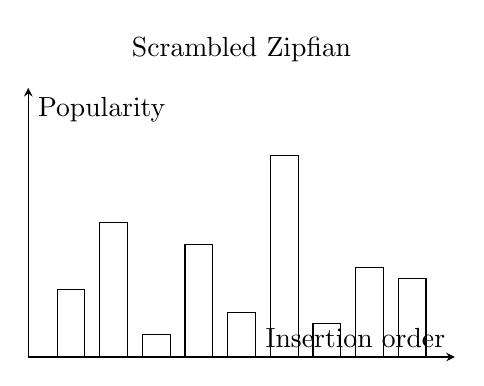
\begin{tikzpicture}
        \begin{axis}[
            width=7cm,
            height=5cm,
            title={Scrambled Zipfian},
            xlabel style={at={(axis description cs:0.5,-0.1)},anchor=north},
            ylabel style={at={(axis description cs:-0.1,.5)},rotate=90,anchor=south},
            xlabel={Insertion order},
            ylabel={Popularity},
            xtick=\empty,
            ytick=\empty,
            axis lines=middle,
            ymin=0, ymax=1.2,
            xmin=0, xmax=10
        ]
        \addplot[ybar,fill=white,draw=black] coordinates {(1,0.3) (2,0.6) (3,0.1) (4,0.5) (5,0.2) (6,0.9) (7,0.15) (8,0.4) (9,0.35)};
        \end{axis}
    \end{tikzpicture}
    \hspace{1cm}
    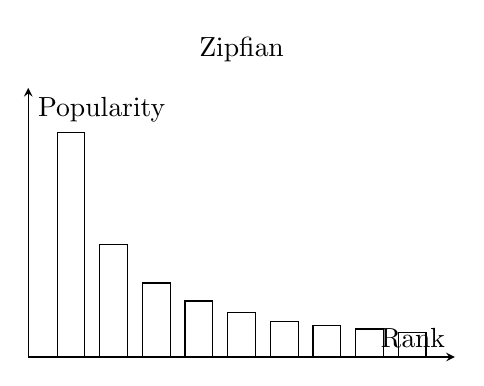
\begin{tikzpicture}
        \begin{axis}[
            width=7cm,
            height=5cm,
            title={Zipfian},
            xlabel style={at={(axis description cs:0.5,-0.1)},anchor=north},
            ylabel style={at={(axis description cs:-0.1,.5)},rotate=90,anchor=south},
            xlabel={Rank},
            ylabel={Popularity},
            xtick=\empty,
            ytick=\empty,
            axis lines=middle,
            ymin=0, ymax=1.2,
            xmin=0, xmax=10
        ]
        \addplot[ybar,fill=white,draw=black] coordinates {(1,1) (2,0.5) (3,0.33) (4,0.25) (5,0.2) (6,0.16) (7,0.14) (8,0.125) (9,0.11)};
        \end{axis}
    \end{tikzpicture}
    \caption{Comparison of Jim Gray's version (right) and the one employed by YCSB (left).}
    \label{fig:zipfian_comparison_ycsb}
\end{figure}

To go around this issue, YCSB uses a hashing algorithm to randomly spread the values in the range as well as employing an extended domain to reduce collisions~\cite{cooperBenchmarkingCloudServing2010}. 

\begin{figure}[htbp]
  \centering
  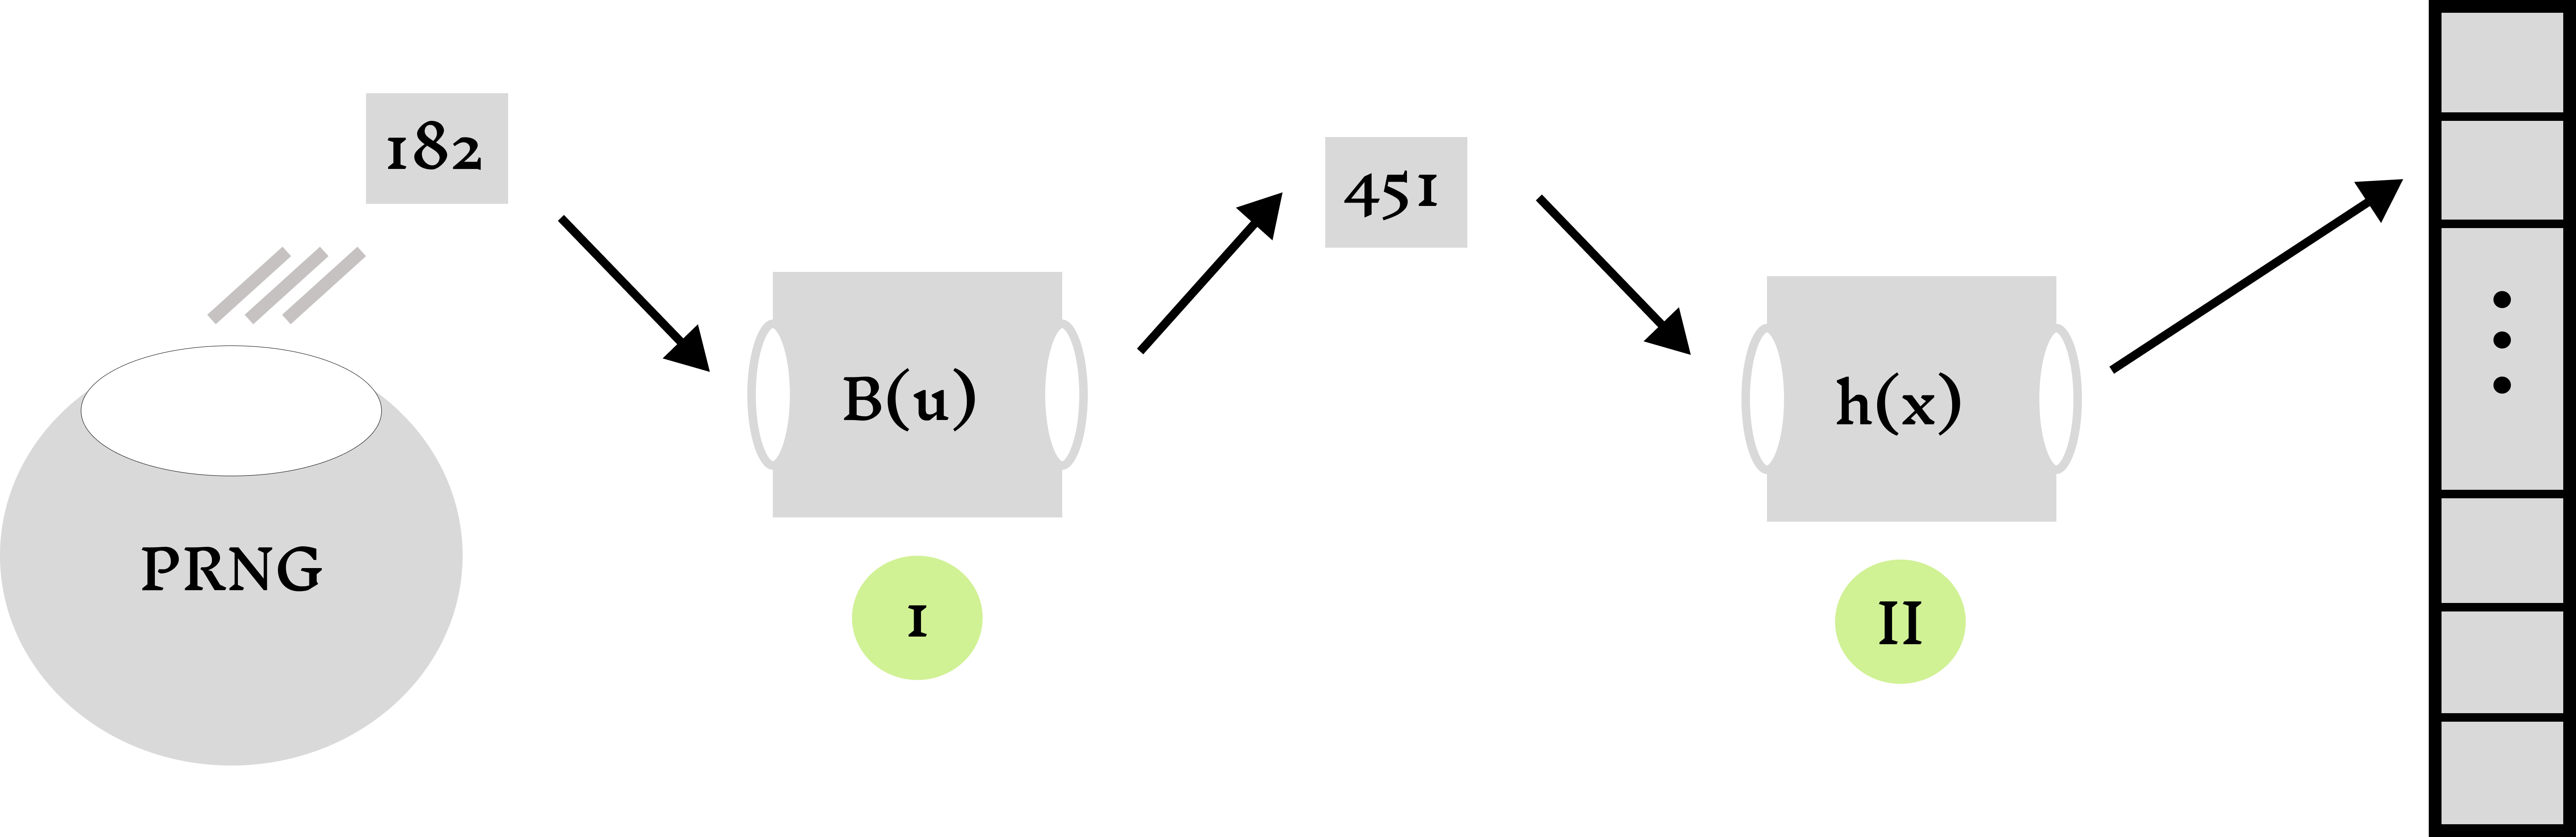
\includegraphics[width=\linewidth]{figures/explanation_ycsb.png}
  \caption{YCSB does sampling by inversion (1) and then hashes the value to spread in in the available range (2)}
  \label{fig:explanation_rej_samp}
\end{figure}

\subsection{Flexible I/O Tester}
\ac{FIO} \cite{1FioFlexible} is a benchmarking tool for storage systems. Much like YCSB, its purpose is generating workloads following a certain pattern access
to test a storage system. The workloads can vary in type, including sequential or random and read-only, write-only or mixed. In the case of \textbf{random I/O} , the user is able to 
to change the access pattern with the goal of simulating both asymetrical and more symmetrical workloads. The underlying distributions include:
\begin{itemize}
  \item Zipfian 
  \item Normal
  \item Pareto
  \item Uniform
\end{itemize}

The generation of a Zipfian distribution works by the same principle as YCSB, meaning:
\begin{enumerate}
  \item Generate a zipfian variate using the algorithm proposed by Jim Gray \cite{grayQuicklyGeneratingBillionrecord1994}
  \item Hash the value to spread it in the range
\end{enumerate}

The same principle applies as in \ref{fig:explanation_rej_samp}

\subsection{Sysbench}
Sysbench \cite{kopytovAkopytovSysbench2025} is a benchmarking tool for databases as well as storages systems. It works in a manner
very similar to YCSB, using multi-threading to strain the system with concurrent accesses. The tool is capable of generating synthetic data
according to different probability distributions, among which the Zipfian distribution.

What sets it apart from the previous ones is that the variate generation uses a different algorithm. The one employed by Sysbench is based on a paper
by Wolfgang Hörmann \cite{hormannRejectioninversionGenerateVariates1996} and the implementation is based off the Apache Commons Math library \cite{MathCommonsMath}, under the 
name \textit{RejectionInversionZipfSampler}.

\subsection{OLTP-Bench}
The OLTP-Bench \cite{difallahOLTPBenchExtensibleTestbed2013} strives to unify different types of benchmarks for evaluating a given \ac{DBMS}. It favours a modular design, enabling very different benchmarks
to be used under a common interface, which makes it quite extensible. However, it also has enough benchmarks built-in to be used directly, among which:
\begin{itemize}
  \item AuctionMark \cite{AuctionMarkOLTPBenchmark}
  \item \ac{TPC-C}
  \item \ac{YCSB}
\end{itemize}

The focus will be rather layed upon the AuctionMark benchmark as it's the one excepting \ac{YCSB} which generates synthetic
data following a Zipfian distribution. The implementation is based on an inverse transformation sampling sped up by a binary search.

% TODO : Remove DBGen from the paper, it's too vague a concept to be called a framework